\section{Mapzen}
\subsection{Tambahkan shapefile OSM2PGSQL ke QGIS}
Cara menambahkan shapfile OSM2PGSQL ke QGIS:
\begin{enumerate}
\item Jalankan QGIS dan tampilkan peta kosong.
\item Pada panel Browser, navigasikan ke folder dimana shapefile disimpan dan buka file 'bandung_indonesia.osm2pgsql-shapefiles'.
\item Perhatikan bahwa file tersebut berisi tiga shapefile, dinamai dengan tipe geometri: line, point ,dan polygon.
\item Klik dua kali pada layer line untuk membukanya di peta. contoh yang di klik adalah 'bandung_indonesia_osm_line'. \ref{micin1}
\begin{figure}[ht]
	\centerline{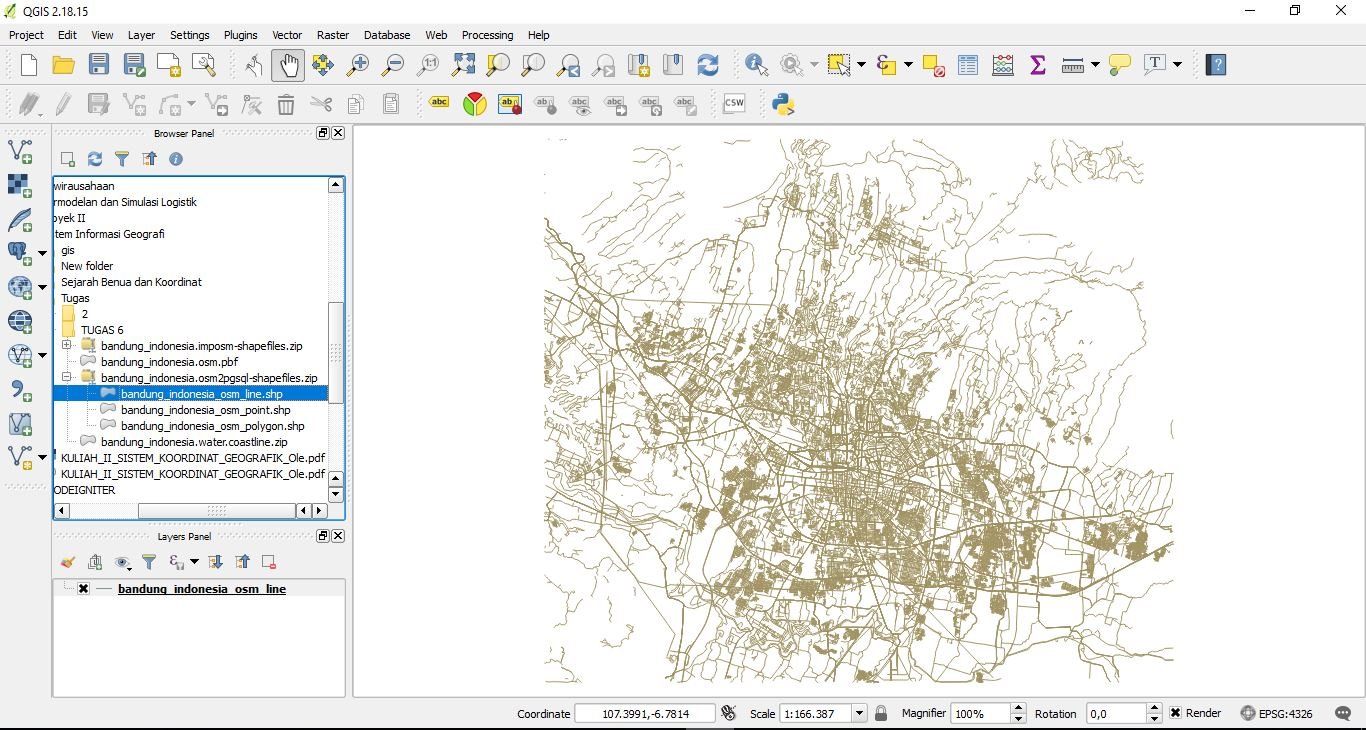
\includegraphics[width=1\textwidth]{figures/micin1.JPG}}
	\caption{OSM2PGSQL ke QGIS}
	\label{micn1}
	\end{figure}
